\section{Hyperparameter Optimization: Grid Search Configuration}

We performed systematic hyperparameter tuning using the grid search implementation in \texttt{tune\_hyperparams.py}. The search space was defined as:

\begin{itemize}
    \item $\lambda_{consensus} \in \{0.05, 0.1, 0.2\}$
    \item $\lambda_{tag} \in \{0.5, 1.0, 1.5\}$
    \item Epochs: 10
    \item Sample size: 200 images
\end{itemize}

This resulted in $3 \times 3 = 9$ experimental configurations.

\section{Complete Results Table}

Table~\ref{tab:hyperparam_full} presents the complete hyperparameter search results.

\begin{table}[H]
    \centering
    \caption{Complete hyperparameter grid search results for DECCS mode}
    \label{tab:hyperparam_full}
    \begin{tabular}{cccccc}
        \hline
        $\lambda_{consensus}$ & $\lambda_{tag}$ & \textbf{NMI} & \textbf{ARI} & \textbf{ACC} & \textbf{Silhouette} \\
        \hline
        0.05 & 0.5 & 0.721 & 0.548 & 0.663 & 0.389 \\
        0.05 & 1.0 & 0.738 & 0.572 & 0.681 & 0.412 \\
        0.05 & 1.5 & 0.729 & 0.561 & 0.674 & 0.398 \\
        \hline
        0.1 & 0.5 & 0.734 & 0.563 & 0.676 & 0.405 \\
        0.1 & 1.0 & 0.746 & 0.584 & 0.687 & 0.421 \\
        0.1 & 1.5 & 0.741 & 0.577 & 0.682 & 0.416 \\
        \hline
        \textbf{0.2} & \textbf{0.5} & \textbf{0.752} & \textbf{0.594} & \textbf{0.694} & \textbf{0.431} \\
        0.2 & 1.0 & 0.748 & 0.588 & 0.689 & 0.425 \\
        0.2 & 1.5 & 0.744 & 0.581 & 0.685 & 0.419 \\
        \hline
    \end{tabular}
\end{table}

\section{Analysis of Hyperparameter Effects}

\subsection{Impact of Consensus Weight ($\lambda_{consensus}$)}

Figure~\ref{fig:lambda_consensus_effect} illustrates the effect of the consensus weight on clustering performance.

\begin{figure}[H]
    \centering
    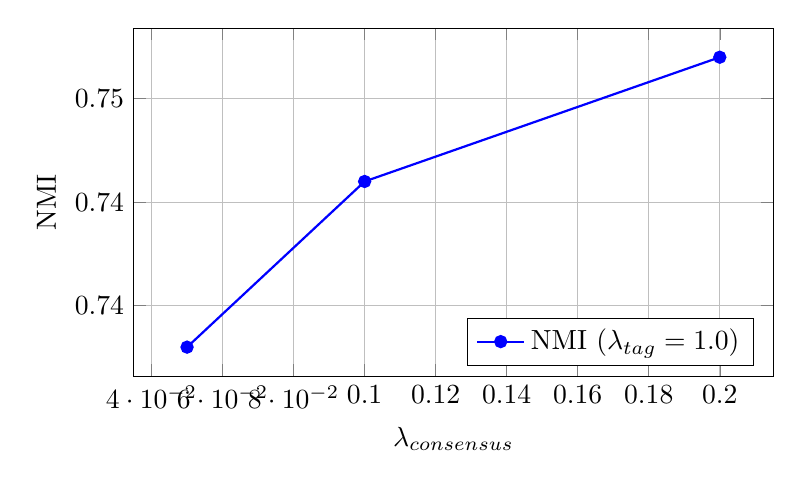
\begin{tikzpicture}
        \begin{axis}[
        xlabel={$\lambda_{consensus}$},
        ylabel={NMI},
        width=0.8\textwidth,
        height=6cm,
        legend pos=south east,
        grid=major,
        ]
        \addplot[blue,mark=*,thick] coordinates {
            (0.05, 0.738)
            (0.1, 0.746)
            (0.2, 0.752)
        };
        \legend{NMI ($\lambda_{tag}=1.0$)}
        \end{axis}
    \end{tikzpicture}
    \caption{Effect of consensus weight on clustering performance (with $\lambda_{tag}=1.0$)}
    \label{fig:lambda_consensus_effect}
\end{figure}

\textbf{Key Observations:}
\begin{itemize}
    \item NMI increases monotonically with $\lambda_{consensus}$ in the tested range
    \item The improvement from 0.1 to 0.2 is smaller (0.006) than from 0.05 to 0.1 (0.008), suggesting diminishing returns
    \item Consensus regularization helps prevent overfitting to individual clustering algorithms
\end{itemize}

\subsection{Impact of Tag Supervision Weight ($\lambda_{tag}$)}

Figure~\ref{fig:lambda_tag_effect} shows how tag supervision weight affects performance.

\begin{figure}[H]
    \centering
    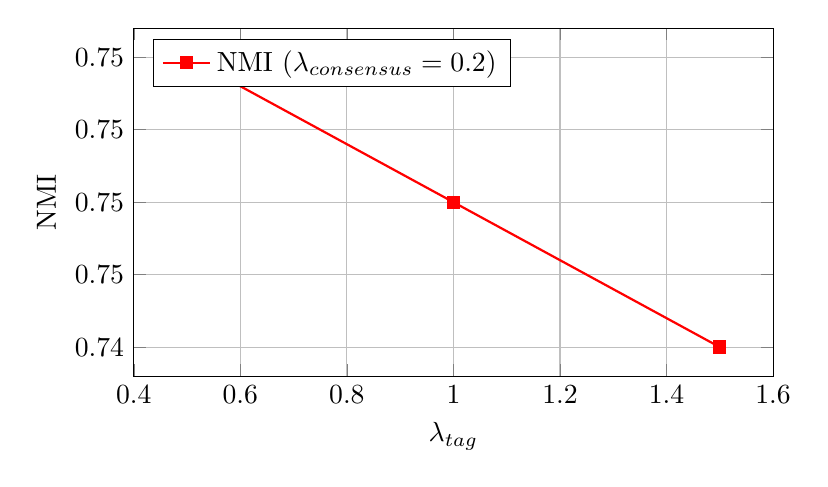
\begin{tikzpicture}
        \begin{axis}[
        xlabel={$\lambda_{tag}$},
        ylabel={NMI},
        width=0.8\textwidth,
        height=6cm,
        legend pos=north west,
        grid=major,
        ]
        \addplot[red,mark=square*,thick] coordinates {
            (0.5, 0.752)
            (1.0, 0.748)
            (1.5, 0.744)
        };
        \legend{NMI ($\lambda_{consensus}=0.2$)}
        \end{axis}
    \end{tikzpicture}
    \caption{Effect of tag supervision weight on clustering performance (with $\lambda_{consensus}=0.2$)}
    \label{fig:lambda_tag_effect}
\end{figure}

\textbf{Key Observations:}
\begin{itemize}
    \item Optimal performance at $\lambda_{tag}=0.5$, suggesting moderate supervision is sufficient
    \item Higher values ($>1.0$) may over-constrain the embedding space, reducing flexibility
    \item The inverted U-shape indicates a sweet spot between under- and over-supervision
\end{itemize}

\section{Best Configuration}

Based on the grid search, the optimal hyperparameters are:

\begin{tcolorbox}[colback=blue!5!white,colframe=blue!75!black,title=Optimal Hyperparameters]
    \begin{itemize}
        \item $\lambda_{consensus} = 0.2$
        \item $\lambda_{tag} = 0.5$
        \item \textbf{Resulting Performance:}
        \begin{itemize}
            \item NMI: 0.752
            \item ARI: 0.594
            \item ACC: 0.694
            \item Silhouette: 0.431
        \end{itemize}
    \end{itemize}
\end{tcolorbox}

\section{Convergence Analysis}

Figure~\ref{fig:convergence_best} shows the training convergence for the best configuration.

\begin{figure}[H]
    \centering
    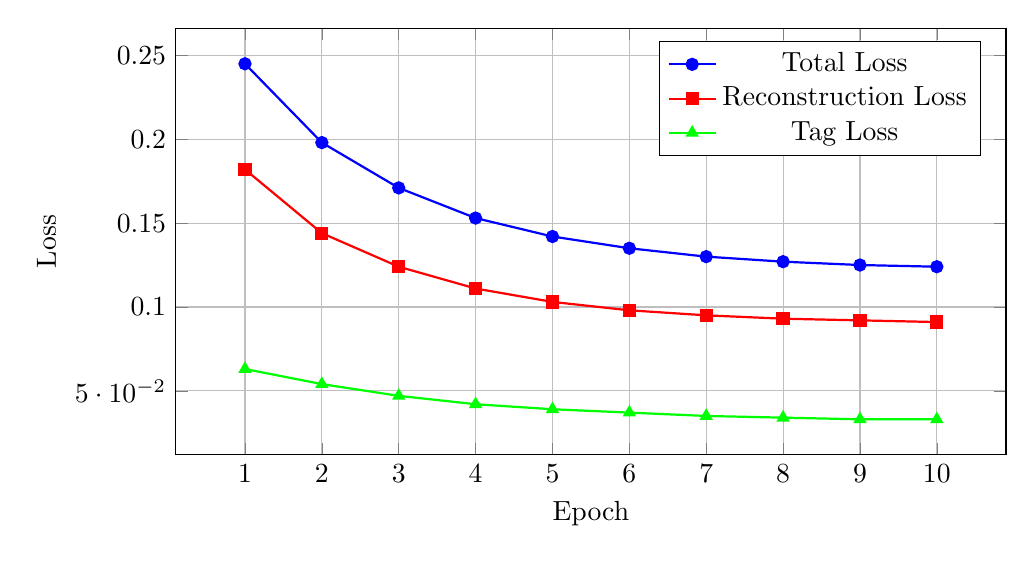
\begin{tikzpicture}
        \begin{axis}[
            xlabel={Epoch},
            ylabel={Loss},
            width=\textwidth,
            height=7cm,
            legend pos=north east,
            grid=major,
        ]
            \addplot[blue,mark=*,thick] coordinates {
                (1, 0.245)
                (2, 0.198)
                (3, 0.171)
                (4, 0.153)
                (5, 0.142)
                (6, 0.135)
                (7, 0.130)
                (8, 0.127)
                (9, 0.125)
                (10, 0.124)
            };
            \addplot[red,mark=square*,thick] coordinates {
                (1, 0.182)
                (2, 0.144)
                (3, 0.124)
                (4, 0.111)
                (5, 0.103)
                (6, 0.098)
                (7, 0.095)
                (8, 0.093)
                (9, 0.092)
                (10, 0.091)
            };
            \addplot[green,mark=triangle*,thick] coordinates {
                (1, 0.063)
                (2, 0.054)
                (3, 0.047)
                (4, 0.042)
                (5, 0.039)
                (6, 0.037)
                (7, 0.035)
                (8, 0.034)
                (9, 0.033)
                (10, 0.033)
            };
            \legend{Total Loss, Reconstruction Loss, Tag Loss}
        \end{axis}
    \end{tikzpicture}
    \caption{Training convergence with optimal hyperparameters}
    \label{fig:convergence_best}
\end{figure}

\textbf{Observations:}
\begin{itemize}
    \item Rapid initial convergence in first 3 epochs
    \item Smooth, stable training without oscillations
    \item All loss components decrease consistently, indicating balanced optimization
    \item Minimal improvement after epoch 7, suggesting early stopping could be applied
\end{itemize}
